\PassOptionsToPackage{unicode=true}{hyperref} % options for packages loaded elsewhere
\PassOptionsToPackage{hyphens}{url}
%
\documentclass[ignorenonframetext,]{beamer}
\usepackage{pgfpages}
\setbeamertemplate{caption}[numbered]
\setbeamertemplate{caption label separator}{: }
\setbeamercolor{caption name}{fg=normal text.fg}
\beamertemplatenavigationsymbolsempty
% Prevent slide breaks in the middle of a paragraph:
\widowpenalties 1 10000
\raggedbottom
\setbeamertemplate{part page}{
\centering
\begin{beamercolorbox}[sep=16pt,center]{part title}
  \usebeamerfont{part title}\insertpart\par
\end{beamercolorbox}
}
\setbeamertemplate{section page}{
\centering
\begin{beamercolorbox}[sep=12pt,center]{part title}
  \usebeamerfont{section title}\insertsection\par
\end{beamercolorbox}
}
\setbeamertemplate{subsection page}{
\centering
\begin{beamercolorbox}[sep=8pt,center]{part title}
  \usebeamerfont{subsection title}\insertsubsection\par
\end{beamercolorbox}
}
\AtBeginPart{
  \frame{\partpage}
}
\AtBeginSection{
  \ifbibliography
  \else
    \frame{\sectionpage}
  \fi
}
\AtBeginSubsection{
  \frame{\subsectionpage}
}
\usepackage{lmodern}
\usepackage{amssymb,amsmath}
\usepackage{ifxetex,ifluatex}
\usepackage{fixltx2e} % provides \textsubscript
\ifnum 0\ifxetex 1\fi\ifluatex 1\fi=0 % if pdftex
  \usepackage[T1]{fontenc}
  \usepackage[utf8]{inputenc}
  \usepackage{textcomp} % provides euro and other symbols
\else % if luatex or xelatex
  \usepackage{unicode-math}
  \defaultfontfeatures{Ligatures=TeX,Scale=MatchLowercase}
\fi
% use upquote if available, for straight quotes in verbatim environments
\IfFileExists{upquote.sty}{\usepackage{upquote}}{}
% use microtype if available
\IfFileExists{microtype.sty}{%
\usepackage[]{microtype}
\UseMicrotypeSet[protrusion]{basicmath} % disable protrusion for tt fonts
}{}
\IfFileExists{parskip.sty}{%
\usepackage{parskip}
}{% else
\setlength{\parindent}{0pt}
\setlength{\parskip}{6pt plus 2pt minus 1pt}
}
\usepackage{hyperref}
\hypersetup{
            pdftitle={Basics of Quantitative Genetics},
            pdfauthor={Peter von Rohr},
            pdfborder={0 0 0},
            breaklinks=true}
\urlstyle{same}  % don't use monospace font for urls
\newif\ifbibliography
\usepackage{longtable,booktabs}
\usepackage{caption}
% These lines are needed to make table captions work with longtable:
\makeatletter
\def\fnum@table{\tablename~\thetable}
\makeatother
\usepackage{graphicx,grffile}
\makeatletter
\def\maxwidth{\ifdim\Gin@nat@width>\linewidth\linewidth\else\Gin@nat@width\fi}
\def\maxheight{\ifdim\Gin@nat@height>\textheight\textheight\else\Gin@nat@height\fi}
\makeatother
% Scale images if necessary, so that they will not overflow the page
% margins by default, and it is still possible to overwrite the defaults
% using explicit options in \includegraphics[width, height, ...]{}
\setkeys{Gin}{width=\maxwidth,height=\maxheight,keepaspectratio}
\setlength{\emergencystretch}{3em}  % prevent overfull lines
\providecommand{\tightlist}{%
  \setlength{\itemsep}{0pt}\setlength{\parskip}{0pt}}
\setcounter{secnumdepth}{0}

% set default figure placement to htbp
\makeatletter
\def\fps@figure{htbp}
\makeatother


\title{Basics of Quantitative Genetics}
\author{Peter von Rohr}
\date{27 September 2019}

\begin{document}
\frame{\titlepage}

\begin{frame}{Background}
\protect\hypertarget{background}{}

\begin{itemize}
\tightlist
\item
  Central Dogma of Molecular Biology
\end{itemize}

\(\rightarrow\) Genotypes are the basis for phenotypic expression

\begin{itemize}
\tightlist
\item
  Start with simple model
\end{itemize}

\(\rightarrow\) one locus that affects quantitative trait

\end{frame}

\begin{frame}{Population}
\protect\hypertarget{population}{}

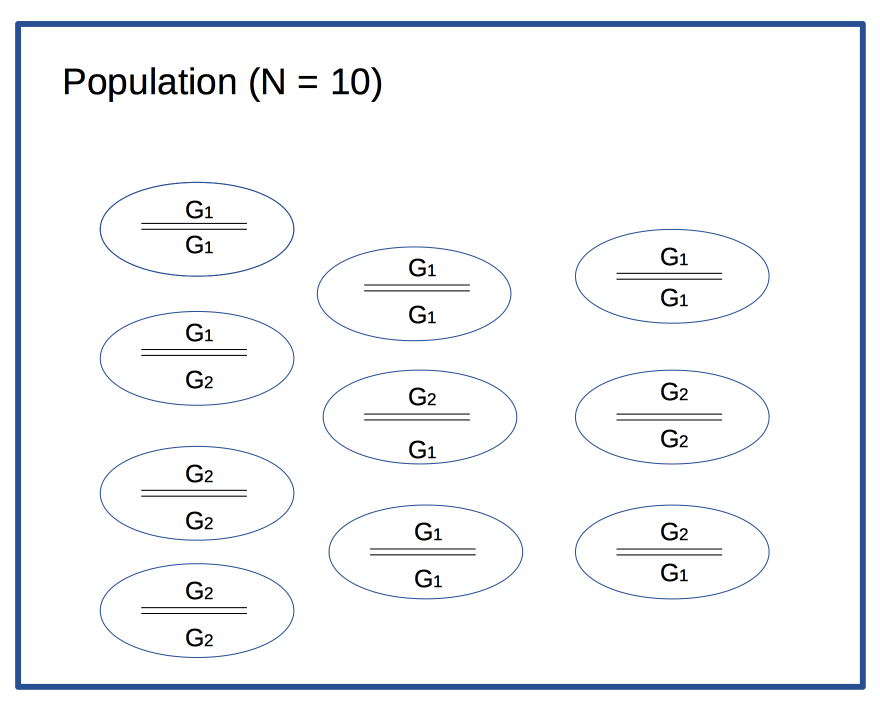
\includegraphics{odg/idealpopsingletrait.png}

\end{frame}

\begin{frame}{Terminology}
\protect\hypertarget{terminology}{}

\begin{itemize}
\tightlist
\item
  \textbf{alleles}: variants occuring at a given genetic Locus
\item
  \textbf{bi-allelic}: only two alleles, e.g., \(G_1\) and \(G_2\) at a
  given locus \(G\) in population
\item
  \textbf{genotype}: combination of two alleles at locus \(G\) in an
  individual
\item
  \textbf{homozygous}: genotypes \(G_1G_1\) and \(G_2G_2\) where both
  alleles identical
\item
  \textbf{heterozygous}: genotype \(G_1G_2\) different alleles
\end{itemize}

\end{frame}

\begin{frame}{Frequencies in Example Population}
\protect\hypertarget{frequencies-in-example-population}{}

\begin{itemize}
\item
  \textbf{genotype frequencies} \vspace{-2ex} \begin{align}
  f(G_1G_1) &= \frac{4}{10} = 0.4 \notag \\
  f(G_1G_2) &= \frac{3}{10} = 0.3 \notag \\
  f(G_2G_2) &= \frac{3}{10} = 0.3 \notag
  \end{align}
\item
  \textbf{allele frequencies} \vspace{-2ex} \begin{align}
  f(G_1) &= f(G_1G_1) + {1\over 2}*f(G_1G_2) = 0.55 \notag \\
  f(G_2) &= f(G_2G_2) + {1\over 2}*f(G_1G_2) = 0.45 \notag
  \end{align}
\end{itemize}

\end{frame}

\begin{frame}{Hardy-Weinberg Equilibrium}
\protect\hypertarget{hardy-weinberg-equilibrium}{}

\begin{itemize}
\item
  \textbf{allele frequencies} \begin{equation}
  f(G_1) = p  \text{, } f(G_2) = q = 1-p \notag
  \end{equation}
\item
  \textbf{genotype frequencies}
\end{itemize}

\begin{longtable}[]{@{}ccc@{}}
\toprule
Alleles & \(G_1\) & \(G_2\)\tabularnewline
\midrule
\endhead
\(G_1\) & \(f(G_1G_1) = p^2\) & \(f(G_1G_2) = p*q\)\tabularnewline
\(G_2\) & \(f(G_1G_2) = p*q\) & \(f(G_2G_2) = q^2\)\tabularnewline
\bottomrule
\end{longtable}

\begin{equation}
f(G_1G_1) = p^2 \text{, } f(G_1G_2) = 2pq  \text{, } f(G_2G_2) = q^2 \notag
\end{equation}

\end{frame}

\begin{frame}{Genotypic Values}
\protect\hypertarget{genotypic-values}{}

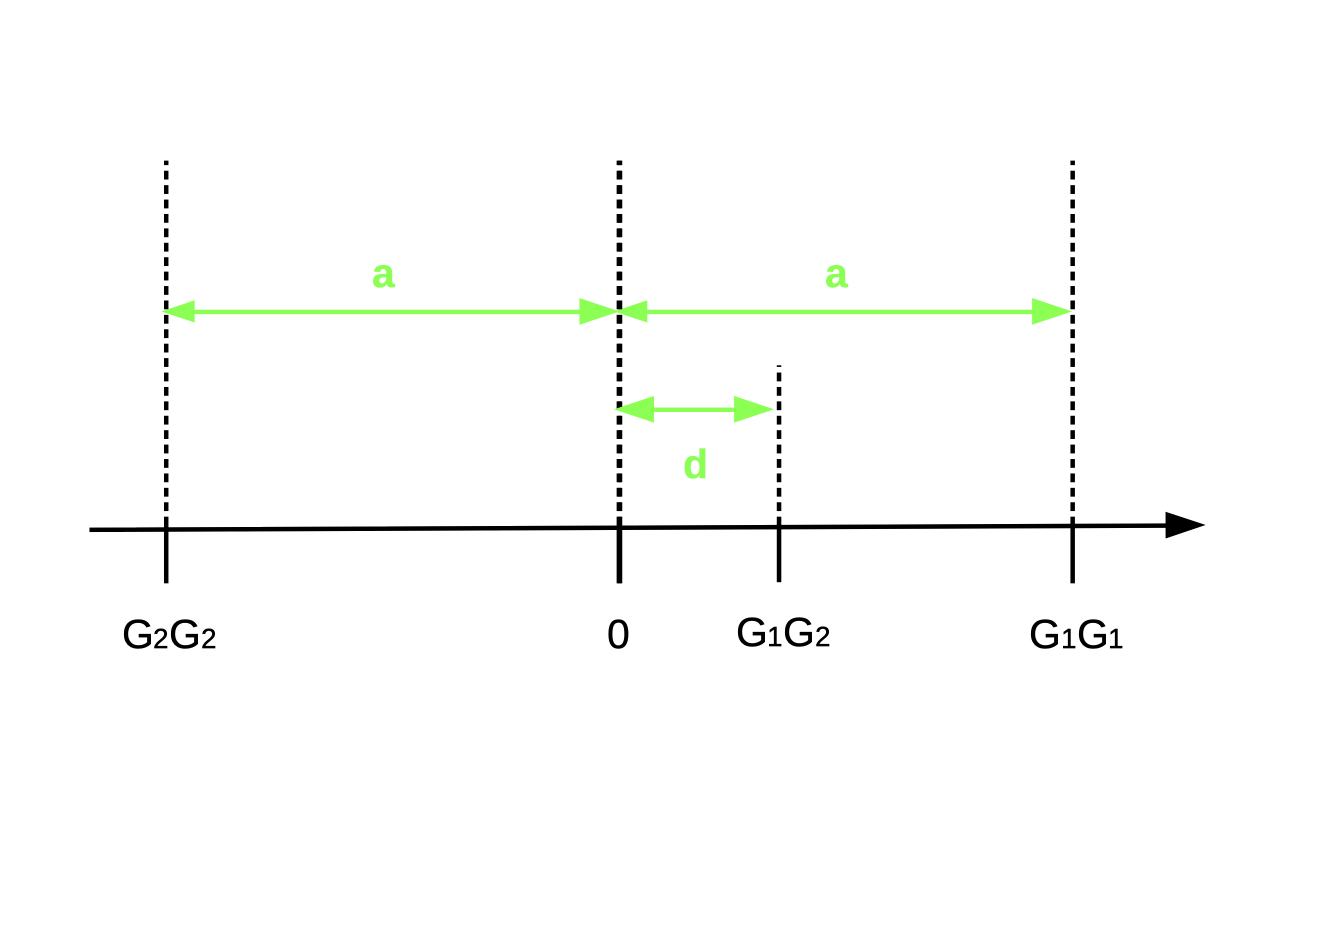
\includegraphics{odg/genotypicvalue.png}

\end{frame}

\begin{frame}{Population Mean}
\protect\hypertarget{population-mean}{}

\begin{itemize}
\tightlist
\item
  Expected value of genotypic value \(V\) as discrete random variable
\end{itemize}

\begin{align}
\mu &= V_{11} * f(G_1G_1) + V_{12} * f(G_1G_2) + V_{22} * f(G_2G_2) \notag \\
    &= a * p^2 + d *2pq + (-a) * q^2 \notag \\
    &= (p-q)a + 2pqd \notag
\end{align}

\end{frame}

\begin{frame}{Breeding Values Definition}
\protect\hypertarget{breeding-values-definition}{}

The breeding value of an animal \(i\) is defined as two times the
difference between the mean value of offsprings of animal \(i\) and the
population mean.

\end{frame}

\begin{frame}{Derivation of Breeding value for \(G_1G_1\)}
\protect\hypertarget{derivation-of-breeding-value-for-g_1g_1}{}

\begin{center}
   {\renewcommand{\arraystretch}{1.7}
   \renewcommand{\tabcolsep}{0.2cm}
   \begin{tabular}{|c|c|c|}
\hline
& \multicolumn{2}{|c|}{Mates of $S$} \\
\hline
& $f(G_1) = p$       &  $f(G_2) = q$   \\
\hline
Parent $S$       &                    &                 \\
\hline
$f(G_1) = 1$ &  $f(G_1G_1) = p$   &  $f(G_1G_2) = q$\\
\hline
\end{tabular}}
\end{center}

\end{frame}

\begin{frame}{Computation of Breeding value for \(G_1G_1\)}
\protect\hypertarget{computation-of-breeding-value-for-g_1g_1}{}

\begin{equation}
\mu_{11} = p*a + q*d \notag
\end{equation}

The breeding value \(BV_{11}\) corresponds to

\begin{align}
BV_{11} &=  2*(\mu_{11} - \mu)  \notag \\
        &=  2\left(pa + qd - \left[(p - q)a + 2pqd \right] \right) \notag\\
        &=  2\left(pa + qd - (p - q)a - 2pqd \right) \notag\\
        &=  2\left(qd + qa - 2pqd\right) \notag \\
        &=  2\left(qa + qd(1 - 2p)\right) \notag \\
        &=  2q\left(a + d(1 - 2p)\right) \notag \\
        &=  2q\left(a + (q-p)d\right) \notag
\end{align}

\end{frame}

\begin{frame}{Computation of Breeding value for \(G_2G_2\)}
\protect\hypertarget{computation-of-breeding-value-for-g_2g_2}{}

\begin{equation}
\mu_{22} = pd - qa \notag
\end{equation}

The breeding value \(BV_{22}\) corresponds to

\begin{align}
BV_{22} &=   2*(\mu_{22} - \mu)  \notag \\
        &=   2\left(pd - qa - \left[(p - q)a + 2pqd \right] \right) \notag \\
        &=   2\left(pd - qa - (p - q)a - 2pqd \right) \notag \\
        &=   2\left(pd - pa - 2pqd\right) \notag \\
        &=   2\left(-pa + p(1-2q)d\right) \notag \\
        &=  -2p\left(a + (q - p)d\right) \notag
\end{align}

\end{frame}

\begin{frame}{Computation of Breeding value for \(G_1G_2\)}
\protect\hypertarget{computation-of-breeding-value-for-g_1g_2}{}

\begin{equation}
\mu_{12} = 0.5pa + 0.5d - 0.5qa = 0.5\left[(p-q)a + d \right] \notag
\end{equation}

The breeding value \(BV_{12}\) corresponds to

\begin{align}
ZW_{12} &=   2*(\mu_{12} - \mu) \notag \\
        &=   2\left(0.5(p-q)a + 0.5d - \left[(p - q)a + 2pqd \right] \right) \notag \\
        &=   2\left(0.5pa - 0.5qa + 0.5d - pa + qa - 2pqd \right) \notag \\
        &=   2\left(0.5(q-p)a + (0.5 - 2pq)d \right) \notag \\
        &=   (q-p)a + (1-4pq)d  \notag \\
        &=   (q-p)a + (p^2 + 2pq + q^2 -4pq)d  \notag \\
        &=   (q-p)a + (p^2 - 2pq + q^2)d  \notag \\
        &=   (q-p)a + (q - p)^2d   \notag \\
        &=   (q-p)\left[a + (q-p)d \right] \notag
\end{align}

\end{frame}

\begin{frame}{Summary of Breeding Values}
\protect\hypertarget{summary-of-breeding-values}{}

\begin{center}

with \(\alpha = a + (q-p)d\)

\end{frame}

\begin{frame}{Allele Substitution}
\protect\hypertarget{allele-substitution}{}

\begin{align}
    BV_{12} - BV_{22} &=   (q-p)\alpha - \left( -2p\alpha \right)  \notag \\
                      &=   (q-p)\alpha + 2p\alpha \notag \\
                      &=   (q-p+2p)\alpha \notag \\
                      &=   (q+p)\alpha \notag \\
                      &=   \alpha \notag
\end{align}

\begin{align}
    BV_{11} - BV_{12} &=   2q\alpha - (q-p)\alpha \nonumber \\
                      &=   \left(2q - (q-p)\right)\alpha \nonumber\\
                      &=   \alpha \notag
\end{align}

\end{frame}

\begin{frame}{Dominance Deviation I}
\protect\hypertarget{dominance-deviation-i}{}

\begin{align}
  V_{11} - BV_{11} &=   a - 2q \alpha \notag \\
                   &=   a - 2q \left[ a + (q-p)d \right] \notag \\
                   &=   a - 2qa -2q(q-p)d \notag \\
                   &=   a(1-2q) - 2q^2d + 2pqd \notag \\
                   &=   \left[(p - q)a + 2pqd\right] - 2q^2d \notag \\
                   &=   \mu + D_{11} \notag
  \end{align}

\end{frame}

\begin{frame}{Dominance Deviation II}
\protect\hypertarget{dominance-deviation-ii}{}

\begin{align}
  V_{12} - BV_{12} &=   d - (q-p)\alpha \notag \\
                   &=   d - (q-p)\left[ a + (q-p)d \right] \notag \\
                   &=   \left[(p-q)a + 2pqd\right] + 2pqd \notag \\
                   &=   \mu + D_{12} \notag
  \end{align}

\begin{align}
  V_{22} - BV_{22} &=   -a - (-2p\alpha) \notag \\
                   &=   -a + 2p\left[ a + (q-p)d \right] \notag \\
                   &=   \left[(p-q)a + 2pqd\right] - 2p^2d \notag \\
                   &=   \mu + D_{22} \notag
  \end{align}

\end{frame}

\begin{frame}{Summary of Values}
\protect\hypertarget{summary-of-values}{}

\begin{tabular}{|c|c|c|c|}
\hline
Genotyp  &  genotypic value     &  Breeding Value    &  Dominance Deviation \\
$G_iG_j$ &  $V_{ij}$            &  $BV_{ij}$         &  $D_{ij}$           \\
\hline
$G_1G_1$ &  $a$                 &  $2q\alpha$        &  $-2q^2d$          \\
\hline
$G_1G_2$ &  $d$                 &  $(q-p)\alpha$     & $2pqd$             \\
\hline
$G_2G_2$ &  $-a$                &  $-2p\alpha$       & $-2p^2d$           \\
\hline
\end{tabular}

\end{frame}

\begin{frame}{Decomposition of Genotypic Values}
\protect\hypertarget{decomposition-of-genotypic-values}{}

\begin{align}
V_{ij} &=   \mu + BV_{ij} + D_{ij} \notag
\end{align}

\end{frame}

\end{document}
